\documentclass[uplatex,dvipdfmx]{jsarticle}

%\usepackage{luatexja}
\usepackage{docmute}

%\usepackage[2.0]{bxpdfver}


\usepackage{graphicx}

\usepackage{xcolor}
\graphicspath{{./docs/images/}{./images/}}
\definecolor{forground}{gray}{0.75}
\definecolor{background}{gray}{0.10}
\color{forground}
\pagecolor{background}

\usepackage{siunitx}

\usepackage{tikz}
\usetikzlibrary{intersections,calc,arrows.meta}

%\usepackage[style=base]{caption}
\usepackage[subrefformat=parens]{subcaption}

\usepackage{prettyref}
\newrefformat{note}{脚注~\ref*{#1}}
\newrefformat{figs}{図~\ref*{#1}}
\newrefformat{fig}{図~\ref*{#1}}
\newrefformat{tbl}{表~\ref*{#1}}
\newcommand*{\fullref}[1]{\hyperref[#1]{\prettyref{#1}}}

\usepackage[pdfusetitle,hidelinks]{hyperref}
\usepackage{pxjahyper}

\newcommand*{\includefig}[5][c]{%
    \begin{minipage}[#1]{#2\linewidth}
        \centering
        \includegraphics[width=\linewidth]{#5}
        \subcaption{#3}
        \label{#4}
    \end{minipage}
}
\newenvironment{imageHere}[2][htbp]{\def\@imageHereTmp{#2}%
    \begin{figure}[#1]
        \centering
}{%  
        \caption{\@imageHereTmp}
        \label{figs:\@imageHereTmp}
    \end{figure}
}

\title{
    コズミックトラベル (編集中) \\
    \large 75th2600内装設計チーフ引き継ぎ
}
\author{75th621 千葉森生}
\date{最終更新日: \today}

\begin{document}

\maketitle

\section{まえがき}

入試を間近に控えておきながら今更2年生の引き継ぎを書いているのは、3年のはいいから2年の時の引き継ぎをかけと急かされている私、内設チのライド担当の千葉でございます。

軽くプロフィール(肩書き自慢)を書くと、以下のようになります。
\begin{itemize}
    \item 75th2600, 3600内装設計チーフ
    \item 75th2600原案班
    \item エンジニアチームCTO
    \item 帰宅部 etc...
\end{itemize}

で、どんな内装を作ったかと言いますと、

\begin{imageHere}{設計概観}
    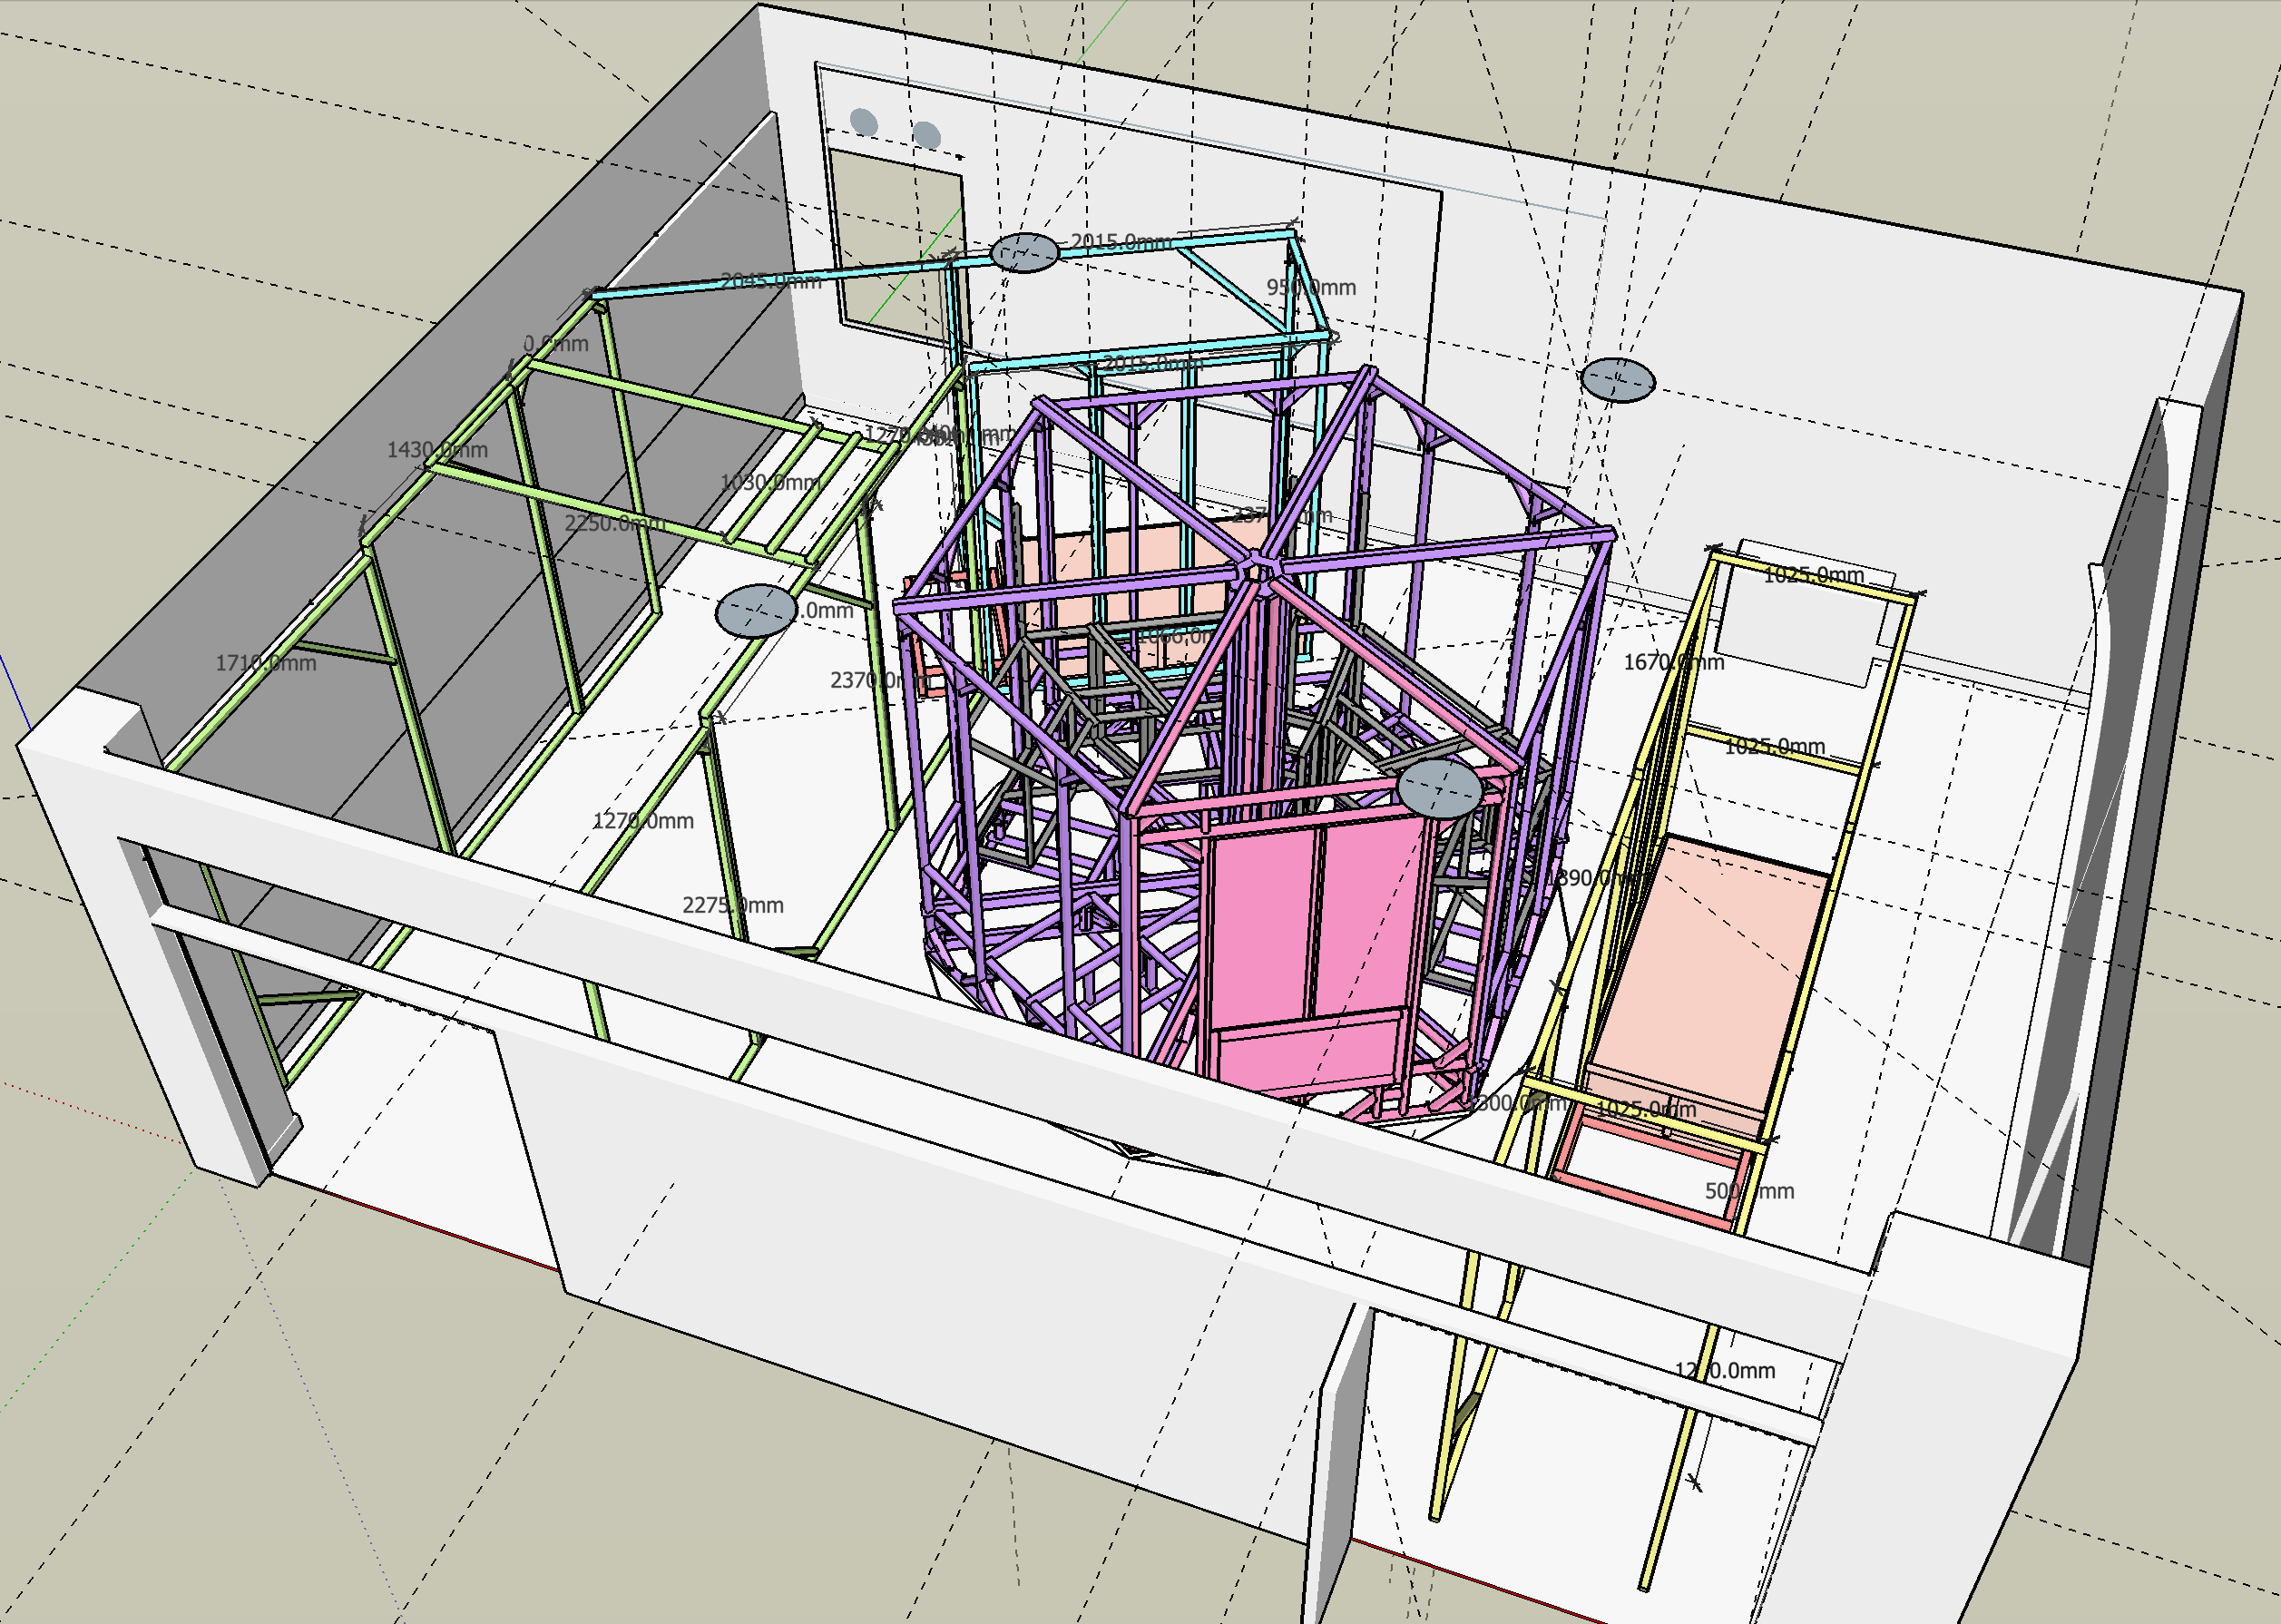
\includegraphics[width=0.5\linewidth]{images/plan_overview/1.png}
\end{imageHere}

こんなのです。真ん中の正六角形の宇宙船に人を2,3人乗せて回しました。そのため、その辺りの補強が割とエグいです。
今後ライドをやるクラスの参考になれば幸いです。
なお、設計チーフの身ながら内チの仕事に近いところまで手を伸ばしていたので、割と手広い引き継ぎになってます。

デザインが論文っぽいのは\LaTeX{}で書いてるからです。あと、資料は全部別ファイルで添付して、一部のみ引用してきてます。詳しく見たければ添付ファイルへgo。

\clearpage

\tableofcontents

\section{TL;DR}
TL;DRってIT界隈でしか通じないらしいですね。Too Long, Don't Readの略で、要約みたいな意味のスラングです。

で、要約、というか伝えたいこと。主に心構え的なこととか。

\begin{itemize}
    \item デザインを待っていたら設計は終わらない。設チが先導せよ。
    \item 目標は高くもて。ただし周りのアドバイスは聞け。
    \item 外装との連携は忘れずに。双方の進捗を見て人員とか作業スペースとか融通しよう。
    \item 教室測定は念入りに。正確に。細部まで。
\end{itemize}

あと、引き継ぎの内容についてでもそれ以外でも、何か質問があればこちらのメールアドレスまでお気軽に:  chibam496@gmail.com
\end{document}